\documentclass[class=report, float=false, crop=false]{standalone}
%  \usepackage[subpreambles=true]{standalone}

\usepackage{pgf, tikz}
\usetikzlibrary{shapes.misc}
\usetikzlibrary{decorations.pathreplacing}

\tikzset{cross/.style={cross out, draw=black, minimum size=2*(#1-\pgflinewidth), inner sep=0pt, outer sep=0pt},
%default radius will be 1pt. 
cross/.default={0.25pt},
    point/.style={
    thick,
    draw=black,
    cross out,
    inner sep=0pt,
    minimum width=4pt,
    minimum height=4pt,
    },
}

\graphicspath{{figures/images/}}

% \begin{cbunit}

\begin{document}

\chapter{Ellipsoids}
\label{chap:ellipsoids}

Our goal here is to formalise the principle of belonging to an ellipsoid and show how this formalism can be exploited in numerical simulations to determine if and how ellipsoids are overlapping.\\

Please find in \hyperref[appendix:ellipsoids]{appendix \ref{appendix:ellipsoids}} a complete presentation of ellipsoids.

\section{Belonging matrix}

Consider an ellipsoid $\mathcal{A}$ of centre $\vec{v}$, semi-axes $(R_i)_{i=1:3}$ and whose orientation is described by the quaternion $q$.\\

In the Euclidean 3D projective space, we can characterise the belonging to this ellipsoid with the mean of a matrix $B(\vec{v},q,(R_i)_{i=1:3}) \in \mathcal{M}_{4}(\mathbb{R})$ with the following properties
\begin{equation}
\forall \vec{r} \in E^3, \begin{cases} \vec{r}^T B \vec{r} < 0 &\text{ if } \vec{r} \in \mathcal{A} \setminus \bar{\mathcal{A}} \\ \vec{r}^T B \vec{r} = 0 &\text{ if } \vec{r} \in \bar{\mathcal{A}} \\ \vec{r}^T B \vec{r} > 0 &\text{ if } \vec{r} \notin \mathcal{A} \end{cases}
\label{belonging_definition_}
\end{equation}
which we will call the \textit{belonging matrix} of the ellipsoid $\mathcal{A}$.\\

Equivalently, we can define in $\mathbb{R}^3$ the matrix
\begin{equation}
\boxed{
\bar{B}(q,(R_i)_{i=1:3}) \equiv \mathcal{Q}_q\text{diag}(R_i^{-2})_{i=1:3}\mathcal{Q}_q^T
}
\label{reduced_belonging_matrix_}
\end{equation}
where $\mathcal{Q}_q$ is the rotation matrix associated with the quaternion $q$, with the following properties
\begin{equation}
\forall \vec{r} \in \mathbb{R}^3, \begin{cases} (\vec{r} - \vec{v})^T \bar{B} (\vec{r} - \vec{v}) < 1 &\text{ if } \vec{r} \in \mathcal{A} \setminus \bar{\mathcal{A}} \\ (\vec{r} - \vec{v})^T \bar{B} (\vec{r} - \vec{v}) = 1 &\text{ if } \vec{r} \in \bar{\mathcal{A}} \\ (\vec{r} - \vec{v})^T \bar{B} (\vec{r} - \vec{v}) > 1 &\text{ if } \vec{r} \notin \mathcal{A} \end{cases}
\label{reduced_belonging_definition_}
\end{equation}
which we will call the \textit{reduced belonging matrix} of the ellipsoid $\mathcal{A}$.\\

From equation \ref{reduced_belonging_definition_}, we can define the function
\begin{equation}
%\boxed{
\begin{aligned}\mathcal{F}_{\mathcal{A}} \colon &\mathbb{R}^3 \to \mathbb{R}\\     &\phantomarrow{\mathbb{R}^3}{\vec{r}} (\vec{r} - \vec{v})^T\bar{B}(q,(R_i)_{i=1:3})(\vec{r}-\vec{v}) - 1\end{aligned}
%}
\label{belonging_function_reduced_}
\end{equation}
which we will call the \textit{belonging function} of the ellipsoid $\mathcal{A}$. This function is linked $\forall \vec{r} \in \mathbb{R}^3$ to the rescaling factor $\mu(\vec{r})$ that has to be applied to $\mathcal{A}$ for $\vec{r}$ to be on its surface
\begin{equation}
\boxed{
\mathcal{F}_{\mathcal{A}}(\vec{r}) = \mu^2(\vec{r}) - 1
}
\end{equation}
Therefore, we have that $\forall \vec{r_S} \in \bar{\mathcal{A}}$, the unit outward-facing normal vector to the ellipsoid in $\vec{r_S}$ is parallel to the gradient of $\mathcal{F}_{\mathcal{A}}(\vec{r_S})$ and has the same direction. We thus have
\begin{equation}
\boxed{
\forall \vec{r_S}\in \bar{\mathcal{A}}, \vec{n}(\vec{r_S}) = \frac{\bar{B}(q,(R_i)_{i=1:3})(\vec{r_S} - \vec{v})}{|\bar{B}(q,(R_i)_{i=1:3})(\vec{r_S} - \vec{v})|}
}
\label{surface_vec_reduced_}
\end{equation}

\section{Separation of ellipsoids}

In this section, we mean to present two methods of determining if two ellipsoids are overlapping. The Wang \textit{et al.} described in part \ref{wang} was considered to be too much time-consuming to be able to implement it in our simulations.\\

We rather decided to implement the Perram and Wertheim method described in part \ref{contact_function_condition}.\\

\subsection{Contact function condition}
\label{contact_function_condition}

\subsubsection{Principle}

The following method was proposed by Perram and Wertheim \cite{perram1985statistical} and was applied to the study of jammed packings of ellipsoidal particles \cite{donev2007underconstrained}. It is extensively described in \cite{donev}, however we will present here a slightly different version, which is closer the original.\\

Consider two ellipsoids $\mathcal{A}$ and $\mathcal{B}$ whose centers are located in $\vec{v}_{\mathcal{A}}$ and $\vec{v}_{\mathcal{B}}$ respectively, $\forall \vec{r} \in \mathbb{R}^3$ we introduce $\mu_{\mathcal{A}}(\vec{r})$ and $\mu_{\mathcal{B}}(\vec{r})$ the rescaling functions of the ellipsoids, \textit{i.e.} the functions that associate to any point $\vec{r}$ the rescaling factor that has to be applied to the ellipsoid for $\vec{r}$ to be on its surface. We then define the \textit{contact function} $F$ such that
\begin{equation}
\forall \vec{r} \in \mathbb{R}^3, \forall \lambda \in [0,1], F(\vec{r},\lambda) = \lambda\mu_{\mathcal{A}}^2(\vec{r}) + (1-\lambda)\mu_{\mathcal{B}}^2(\vec{r})
\label{contact_function}
\end{equation}

According to the authors of \cite{perram1985statistical}, $\forall \lambda \in [0,1]$, $\exists!~ \vec{r}(\lambda) \in \mathbb{R}^3$, $\vec{\nabla}F(\vec{r},\lambda) = 0$, where $\vec{r}(\lambda)$ corresponds to a minimum of the contact function. We can notice that $\vec{r}(\lambda = 0) = \vec{v}_{\mathcal{B}}$, $\vec{r}(\lambda = 1) = \vec{v}_{\mathcal{A}}$ and $\forall \lambda \in ]0,1[$
\begin{equation}
\vec{\nabla}F(\vec{r}(\lambda),\lambda) = 0 \Leftrightarrow \lambda \vec{\nabla}\mu_{\mathcal{A}}^2(\vec{r}(\lambda)) = - (1 - \lambda)  \vec{\nabla}\mu_{\mathcal{B}}^2(\vec{r}(\lambda))
\label{der_contact_function}
\end{equation}
which shows that if the ellipsoids $\mathcal{A}$ and $\mathcal{B}$ are rescaled with the rescaling factor $\mu_{\mathcal{A}}(\vec{r}(\lambda))$ and $\mu_{\mathcal{B}}(\vec{r}(\lambda))$ respectively, then the normal vectors to these ellipsoids in $\vec{r}(\lambda)$ are parallel with opposite directions.\\

The authors of \cite{perram1985statistical} showed that $\left.\frac{d^2F}{d\lambda^2}\right|_{\vec{r} = \vec{r}(\lambda)}$ is negative definite, then $\exists!~ \lambda^*$, $\left.\frac{dF}{d\lambda}\right|_{\vec{r} = \vec{r}(\lambda^*)} = 0$ and it corresponds to a maximum of $F(\vec{r}(\lambda),\lambda)$. We can notice that
\begin{align*}
\left.\frac{dF}{d\lambda}\right|_{\vec{r} = \vec{r}(\lambda^*)} = 0 &\Leftrightarrow \left[\frac{\partial F}{\partial \lambda}(\vec{r},\lambda) + \vec{r}'(\lambda)\cdot\underbrace{\cancel{\vec{\nabla}F(\vec{r},\lambda)}}_{\vec{\nabla}F(\vec{r}(\lambda),\lambda) = 0}\right]_{\vec{r}=\vec{r}(\lambda^*)} = 0\\
&\Leftrightarrow \mu_{\mathcal{A}}^2(\vec{r}(\lambda^*)) - \mu_{\mathcal{B}}^2(\vec{r}(\lambda^*)) = 0\\
&\Leftrightarrow \mu_{\mathcal{A}}^2(\vec{r}(\lambda^*)) = \mu_{\mathcal{A}}^2(\vec{r}(\lambda^*))
\end{align*}
Therefore, there exists a unique point $\vec{r_C} \equiv \vec{r}(\lambda^*)$ for which both ellipsoids $\mathcal{A}$ and $\mathcal{B}$ are externally tangent when rescaled with a common rescaling factor $\mu^2 \equiv \mu_{\mathcal{A}}^2(\vec{r}(\lambda^*)) = \mu_{\mathcal{B}}^2(\vec{r}(\lambda^*))$.\\

From the definition of $F$ in equation \ref{contact_function} we can infer
\begin{equation}
\boxed{\mu^2 = \max_{0<\lambda<1} F(\vec{r}(\lambda),\lambda)}
\end{equation}
This rescaling factor has to be greater than 1 if the ellipsoids are non-overlapping and lesser than 1 if they are overlapping. Therefore, the computation of $\mu$ tells us when $\mathcal{A}$ and $\mathcal{B}$ are overlapping.

\subsubsection{Computation}

According to equation \ref{belonging_function_reduced_} we can rewrite as a function of the reduced belonging matrix $\bar{B}_{\mathcal{A}}$ and $\bar{B}_{\mathcal{B}}$ and position $\vec{r_{\mathcal{A}}}$ and $\vec{r_{\mathcal{B}}}$ of ellipsoids $\mathcal{A}$ and $\mathcal{B}$ the equation \ref{contact_function}
\begin{equation}
\forall \vec{r} \in \mathbb{R}^3, \forall \lambda \in [0,1], F(\vec{r},\lambda) = \lambda(\vec{r}-\vec{r_{\mathcal{A}}})^T\bar{B}_{\mathcal{A}}(\vec{r}-\vec{r_{\mathcal{A}}}) + (1-\lambda)(\vec{r}-\vec{r_{\mathcal{B}}})^T\bar{B}_{\mathcal{B}}(\vec{r}-\vec{r_{\mathcal{B}}})
\label{contact_function_reduced}
\end{equation}
and the equation \ref{der_contact_function}
\begin{align*}
\vec{\nabla}F(\vec{r}(\lambda),\lambda) = 0 &\Leftrightarrow \lambda \bar{B}_{\mathcal{A}}(\vec{r}(\lambda) - \vec{r_{\mathcal{A}}}) = - (1 - \lambda)  \bar{B}_{\mathcal{B}}(\vec{r}(\lambda) - \vec{r_{\mathcal{B}}})
% \\
% &\Leftrightarrow \lambda \bar{B}_{\mathcal{A}}(\vec{r}(\lambda) - \vec{r_{\mathcal{A}}}) + (1 - \lambda) \bar{B}_{\mathcal{B}}(\vec{r}(\lambda) - \vec{r_{\mathcal{A}}}) = (1 - \lambda)\bar{B}_{\mathcal{B}}(\vec{r}_{\mathcal{B}} - \vec{r}_{\mathcal{A}})\\
% &\Leftrightarrow (\lambda\bar{B}_{\mathcal{B}}^{-1}\bar{B}_{\mathcal{A}} + (1-\lambda)\underbrace{\bar{B}_{\mathcal{B}}^{-1}\bar{B}_{\mathcal{B}}}_{\mathclap{\mathbbm{1}_3 = \bar{B}_{\mathcal{A}}^{-1}\bar{B}_{\mathcal{A}}}})(\vec{r}(\lambda) - \vec{r_{\mathcal{A}}}) = (1 - \lambda)(\vec{r_{\mathcal{B}}} - \vec{r_{\mathcal{A}}})\\
% &\Leftrightarrow (\lambda \bar{B}_{\mathcal{B}}^{-1} + (1 - \lambda)\bar{B}_{\mathcal{A}}^{-1})\bar{B}_{\mathcal{A}}(\vec{r}(\lambda) - \vec{r_{\mathcal{A}}}) = (1 - \lambda)(\vec{r_{\mathcal{B}}} - \vec{r_{\mathcal{A}}})
\end{align*}
from which, if we denote
\begin{equation}
Y_{\mathcal{A}\mathcal{B}} \equiv \lambda \bar{B}_{\mathcal{B}}^{-1} + (1 - \lambda)\bar{B}_{\mathcal{A}}^{-1}
\end{equation}
which is a polynomial of degree 3 easy to compute due to the definition of belonging matrix (equation \ref{reduced_belonging_matrix_}), we can infer
\begin{equation}
\begin{aligned}
\vec{r}(\lambda) - \vec{r_{\mathcal{A}}} &= (1 - \lambda)\bar{B}_{\mathcal{A}}^{-1}Y_{\mathcal{A}\mathcal{B}}^{-1}(\vec{r_{\mathcal{B}}} - \vec{r_{\mathcal{A}}})\\
\vec{r}(\lambda) - \vec{r_{\mathcal{B}}} &= - \lambda \bar{B}_{\mathcal{B}}^{—1}Y_{\mathcal{A}\mathcal{B}}^{-1}(\vec{r_{\mathcal{B}}} - \vec{r_{\mathcal{A}}})
\label{rarlrbrl}
\end{aligned}
\end{equation}
We can inject equations \ref{rarlrbrl} in equation \ref{contact_function_reduced}
\begin{align*}
\forall \lambda \in [0,1], F(\vec{r}(\lambda),\lambda) &= \lambda(1 - \lambda)(\vec{r_{\mathcal{B}}} - \vec{r_{\mathcal{A}}})^T\left((1-\lambda)(\bar{B}_{\mathcal{A}}^{-1}Y_{\mathcal{A}\mathcal{B}}^{—1})^T\cancel{\bar{B}_{\mathcal{A}}\bar{B}_{\mathcal{A}}^{-1}} + \lambda(\bar{B}_{\mathcal{B}}^{-1}Y_{\mathcal{A}\mathcal{B}}^{—1})^T\cancel{\bar{B}_{\mathcal{B}}\bar{B}_{\mathcal{B}}^{-1}}\right)Y_{\mathcal{A}\mathcal{B}}^{-1}(\vec{r_{\mathcal{B}}} - \vec{r_{\mathcal{A}}})\\
&= \lambda(1 - \lambda)(\vec{r_{\mathcal{B}}} - \vec{r_{\mathcal{A}}})^T \Big(\underbrace{((1-\lambda)\bar{B}_{\mathcal{A}}^{—1} + \lambda \bar{B}_{\mathcal{B}}^{-1})}_{\cancel{Y_{\mathcal{A}\mathcal{B}}}}\cancel{Y_{\mathcal{A}\mathcal{B}}^{-1}}\Big)^T Y_{\mathcal{A}\mathcal{B}}^{-1}(\vec{r_{\mathcal{B}}} - \vec{r_{\mathcal{A}}})
\end{align*}
which, by consideration that
\begin{align*}
\forall \lambda \in [0,1], Y_{\mathcal{A}\mathcal{B}}^{-1}(\lambda) = \frac{\text{adj}\left(Y_{\mathcal{A}\mathcal{B}}(\lambda)\right)}{\text{det}\left(Y_{\mathcal{A}\mathcal{B}}(\lambda)\right)}
\end{align*}
leads to
\begin{equation}
\boxed{\forall \lambda \in [0,1], F(\vec{r}(\lambda),\lambda) = \frac{p_{\mathcal{A}\mathcal{B}}(\lambda)}{q_{\mathcal{A}\mathcal{B}}(\lambda)} \equiv \frac{\lambda (1 - \lambda) (\vec{r_{\mathcal{B}}} - \vec{r_{\mathcal{A}}})^T\text{adj}\left(Y_{\mathcal{A}\mathcal{B}}(\lambda)\right)(\vec{r_{\mathcal{B}}} - \vec{r_{\mathcal{A}}})}{\text{det}\left(Y_{\mathcal{A}\mathcal{B}}(\lambda)\right)}}
\end{equation}
where adj designates the adjugate matrix -- \textit{i.e.} the transpose of the cofactor matrix --, det the determinant and where $p_{\mathcal{A}\mathcal{B}}$ and $q_{\mathcal{A}\mathcal{B}}$ are polynomials of degree 4 and 3 respectively.\\

Therefore, the parameter $\lambda^*$ for which $F(\vec{r}(\lambda),\lambda)$ is maximum is the unique root of the polynomial
\begin{equation}
h_{\mathcal{A}\mathcal{B}} = p'_{\mathcal{A}\mathcal{B}}q_{\mathcal{A}\mathcal{B}} - p_{\mathcal{A}\mathcal{B}}q'_{\mathcal{A}\mathcal{B}}
\label{hab}
\end{equation}
in the interval ]0,1[, where $h_{\mathcal{A}\mathcal{B}}$ is a polynomial of degree 6.

\subsubsection{Root finding}

We want to find the unique root of the polynomial $h_{\mathcal{A}\mathcal{B}}$ (equation \ref{hab}) in the interval $]0,1[$.\\

To do so, we can use an Householder's method -- in particular the Newton's method or the Halley's method -- for which we will provide a precision $\varepsilon$ such that the root $\lambda^*$ found by the algorithm verifies $|h_{\mathcal{A}\mathcal{B}}(\lambda^*)| \leq \varepsilon$.\\

These methods find a root close to an initial guess. We will choose the root of $F$ we would be looking for if $\mathcal{A}$ and $\mathcal{B}$ were spheres, \textit{i.e.}
\begin{align*}
\Lambda = \frac{R_{\mathcal{A}}}{R_{\mathcal{A}} + R_{\mathcal{B}}}
\end{align*}
with $R_{\mathcal{A}}$ and $R_{\mathcal{B}}$ the longest semi-axes of ellipsoids $\mathcal{A}$ and $\mathcal{B}$, as suggested by Donev \cite{donev}.\\

For an integer $d > 1$, the Householder's method of order $d$ applied to $h_{\mathcal{A}\mathcal{B}}$ has a rate of convergence of $d+1$ and is defined by the sequence $(\lambda_n)_n \in \mathbb{R}^{\mathbb{N}}$ such that
\begin{equation}
\lambda_0 = \Lambda \text{ and } \forall n \in \mathbb{N}, \lambda_{n+1} = \lambda_n + \frac{(1/h_{\mathcal{A}\mathcal{B}})^{(d-1)}(\lambda_n)}{(1/h_{\mathcal{A}\mathcal{B}})^{(d)}(\lambda_n)}
\end{equation}
from which we infer
\begin{equation}
\lambda^* = \lambda_N \text{, where } N = \min(n \in \mathbb{N}, |h_{\mathcal{A}\mathcal{B}}(\lambda_n)| \leq \varepsilon)
\end{equation}

\paragraph{Newton's method}\mbox{}\\

It corresponds to the Householder's method of order 1, therefore
\begin{equation}
\lambda_0 = \Lambda \text{ and } \forall n \in \mathbb{N}, \lambda_{n+1} = \lambda_n - \frac{h_{\mathcal{A}\mathcal{B}}(\lambda_n)}{h'_{\mathcal{A}\mathcal{B}}(\lambda_n)}
\end{equation}

\paragraph{Haley's method}\mbox{}\\

This method has a greater rate of convergence than the Newton's method, however it needs to compute the second derivative of $h_{\mathcal{A}\mathcal{B}}$ in addition to the first derivative.\\

It corresponds to the Householder's method of order 2, therefore
\begin{equation}
\lambda_0 = \Lambda \text{ and } \forall n \in \mathbb{N}, \lambda_{n+1} = \lambda_n - \frac{h_{\mathcal{A}\mathcal{B}}(\lambda_n)}{h'_{\mathcal{A}\mathcal{B}}(\lambda_n)}\left(1 - \frac{h_{\mathcal{A}\mathcal{B}}(\lambda_n)}{h'_{\mathcal{A}\mathcal{B}}(\lambda_n)}\cdot\frac{h''_{\mathcal{A}\mathcal{B}}(\lambda_n)}{2h'_{\mathcal{A}\mathcal{B}}(\lambda_n)}\right)^{-1}
\end{equation}

\paragraph{Error}\mbox{}\\

These methods return, for a given $\varepsilon > 0$, $\lambda^* \in ]0,1[$ such that $|h_{\mathcal{A}\mathcal{B}}(\lambda^*)| \leq \varepsilon$, therefore we can geometrically determine an approximate interval of certainty $err$ of the position of this root

\begin{figure}[h!]
\centering
\includestandalone{figures/tikz/error_householders_method}
\end{figure}

which is given by
\begin{equation}
\boxed{
err = \frac{2\varepsilon}{h'_{\mathcal{A}\mathcal{B}}(\lambda^*)}
}
\end{equation}

\subsubsection{Polynomial computation}

We will use Horner's rule for polynomial computation, which reduces the number of necessary multiplications and results in less numerical instability due to potential substraction of one large number from another \cite{horner}.\\

For a given polynomial $p(x) = \sum_{i = 0}^n a_ix^i$, we define $\forall~x_0$ the sequence $(b_n,\ldots,b_0)$ such that
\begin{equation}
\begin{aligned}
b_n &\coloneqq a_n\\
b_{n-1} &\coloneqq a_{n-1} + b_n x_0\\
&\vdots\\
b_0 &\coloneqq a_0 + b_1x_0
\end{aligned}
\end{equation}
then, $\boxed{b_0 = p(x_0)}$.

\subsection{Algebraic condition}
\label{wang}

The following method is extensively described in \cite{wang2001algebraic}. Contrarily to the method described in part \ref{contact_function_condition} which is essentially numerical, the following method provides a more simple and accurate condition to determine if two ellipsoids are overlapping, according to the authors. This method was used for continuous collision detection between two moving ellipsoids \cite{choi2009continuous}.

\subsubsection{Principle}

Consider two ellipsoids $\mathcal{A}$ and $\mathcal{B}$ whose centers are located in $\vec{v}_{\mathcal{A}}$ and $\vec{v}_{\mathcal{B}}$, whose orientations are described by the unit quaternions $q_A$ and $q_B$ and whose semi-axes are $(R_i^{(\mathcal{A})})_{i=1:3}$ and $(R_i^{(\mathcal{B})})_{i=1:3}$. We then define the \textit{characteristic polynomial} $f$ such that
\begin{equation}
\forall \lambda \in \mathbb{R}, f(\lambda) = \det\left(\lambda B(\vec{v_A},q_A,(R_i^{(\mathcal{A})})_{i=1:3}) + B(\vec{v_B},q_B,(R_i^{(\mathcal{B})})_{i=1:3})\right)
\label{characteristic_polynomial}
\end{equation}

The authors of \cite{wang2001algebraic} showed that\\
\fbox{
\begin{minipage}{0.88\textwidth}
\begin{itemize}
\item[(i)] The \textit{characteristic equation} $f(\lambda) = 0$ always has at least two negative roots.
\item[(ii)] The two ellipsoids are non-overlapping if and only if $f(\lambda) = 0$ has two distinct positive roots.
\item[(iii)] The two ellipsoids touch other externally if and only if $f(\lambda) = 0$ has a positive dooble root.
\end{itemize}
\end{minipage}
}
\mbox{}\\
Note that if $f(\lambda) = 0$ has a positive double root $\lambda_0$, then $\text{rank}(\lambda_0A + B) = 3$ and the homogeneous coordinates of the contact point $X_0$ are given by the unique non-trivial solution of $(\lambda_0A+B)X=0$ \cite{choi2009continuous}.\\

The key to this method is then to determine the sign of the roots of the characteristic equation. This can be easily computed thanks to Sturm's theorem, presented in part \ref{sturm}.

\subsubsection{Sturm's theorem}
\label{sturm}

Sturm's theorem expresses the number of distinct real roots of a polynomial $p \in \mathbb{R}[x]$ located in an interval in terms of the number of changes of signs of the \textit{Sturm's sequence} at the bounds of the interval \cite{wiki:sturm}.\\

The Sturm's sequence of the polynomial $p$ is constructed as following
\begin{equation}
\begin{aligned}
p_0(x) &\coloneqq p(x)\\
p_1(x) &\coloneqq p'(x)\\
p_2(x) &\coloneqq -\text{rem}(p_0,p_1)\\
&\vdots\\
0 &= -\text{rem}(p_{m-1},p_m)
\end{aligned}
\label{sturm_sequence}
\end{equation}
where $\text{rem}(p_i,p_j)$ denotes the remainder of the Euclidean division of $p_i$ by $p_j$.\\

Given that sequence, we will note $\forall \xi \in \bar{\mathbb{R}}$, $\sigma(\xi)$ the number of sign changes (ignoring zeroes) in the sequence $p_0(\xi),\ldots,p_m(\xi)$. Sturm's theorem then states that $\forall a,b \in \mathbb{R}$, $a \neq b$, the number of distinct roots of $p$ in $(a,b]$ is $\sigma(a) - \sigma(b)$ if $a$ nor $b$ is a multiple root of $p$.

\subsubsection{Lagrange polynomial}

We want to use Sturm's theorem presented in part \ref{sturm} on the characteristic polynomial $p$ of equation \ref{characteristic_polynomial}. However, it is easier to construct the Sturm's sequence of equation \ref{sturm_sequence} if we know the coefficients of $p$. We can choose between these two options to do so:
\begin{itemize}
\item[(i)] Formally calculate the $p$ according to equation \ref{characteristic_polynomial} for a symbolic $\lambda$.
\item[(ii)] Determine a Lagrange polynomial \cite{wiki:lagrange} which is equal to $p$.
\end{itemize}
We will show how to use the latter option.\\

Since any belonging matrix $B \in \mathcal{M}_4(\mathbb{R})$, we have $p \in \mathbb{R}_4[x]$. We choose $\lambda_1, \lambda_2, \lambda_3, \lambda_4, \lambda_5 \in \mathbb{R}$ such that $i \neq j \Leftrightarrow \lambda_i \neq \lambda_j$, then
\begin{align*}
p(x) = p_l(x) &\equiv \sum_{i=1}^5 p(\lambda_i) \prod_{\substack{j=1\\j\neq i}}^5 \frac{x - \lambda_j}{\lambda_i - \lambda_j}\\
&= \sum_{i=1}^5 \left(\frac{P(\lambda_i)}{\prod_{\substack{j=1\\j\neq i}}^5 (\lambda_i - \lambda_j)}\right) \underbrace{\prod_{\substack{j=1\\j\neq i}}^5 (x - \lambda_j)}_{\pi_i}
\end{align*}
Indeed, since $p-p_l \in \mathbb{R}_4[x]$ and $(p-p_l)(\lambda_i) = 0~ \forall i \in \llbracket1,5\rrbracket$ then $p-p_l=0 \Leftrightarrow p = p_l$.\\

We can expanse $\pi_i~\forall i \in \llbracket1,5\rrbracket$ with Viète theorem \cite{viete}:
\begin{align*}
\pi_i = \prod_{\substack{j=1\\j\neq i}}^5 (x - \lambda_j) = x^4 - x^3 \sum_{\substack{j=1\\j\neq i}}^5 \lambda_j + x^2 \sum_{\substack{j=1\\j\neq i}}^5 \sum_{\substack{k>j\\k\neq i}} \lambda_j\lambda_k - x \sum_{\substack{j=1\\j\neq i}}^5 \sum_{\substack{k>j\\k\neq i}} \sum_{\substack{l>k\\l\neq i}} \lambda_j\lambda_k\lambda_l + \prod_{\substack{j=1\\j\neq i}}^5 \lambda_j
\end{align*}
and then write
\begin{equation}
\begin{aligned}
p(x) = p_l(x) =~ &x^4\left(\sum_{i=1}^5 \frac{P(\lambda_i)}{\prod_{\substack{j=1\\j\neq i}}^5 (\lambda_i - \lambda_j)}\right) - x^3\left(\sum_{i=1}^5 \frac{P(\lambda_i)}{\prod_{\substack{j=1\\j\neq i}}^5 (\lambda_i - \lambda_j)}\sum_{\substack{j=1\\j\neq i}}^5 \lambda_j\right)\\
&+ x^2 \left(\sum_{i=1}^5 \frac{P(\lambda_i)}{\prod_{\substack{j=1\\j\neq i}}^5 (\lambda_i - \lambda_j)}\sum_{\substack{j=1\\j\neq i}}^5 \sum_{\substack{k>j\\k\neq i}} \lambda_j\lambda_k\right) - x\left(\sum_{i=1}^5 \frac{P(\lambda_i)}{\prod_{\substack{j=1\\j\neq i}}^5 (\lambda_i - \lambda_j)}\sum_{\substack{j=1\\j\neq i}}^5 \sum_{\substack{k>j\\k\neq i}} \sum_{\substack{l>k\\l\neq i}} \lambda_j\lambda_k\lambda_l\right)\\
&+ \sum_{i=1}^5 \frac{P(\lambda_i)}{\prod_{\substack{j=1\\j\neq i}}^5 (\lambda_i - \lambda_j)}\prod_{\substack{j=1\\j\neq i}}^5 \lambda_j
\end{aligned}
\end{equation}

\section{Distance between two ellipsoids}
\label{distance}

\subsection{Presentation of the problem}

Consider two ellipsoids $\mathcal{A}$ and $\mathcal{B}$, the distance between these ellipsoids is the positive real number $d(\mathcal{A},\mathcal{B})$ defined as
\begin{equation}
d(\mathcal{A},\mathcal{B}) = \begin{cases} \min_{\vec{r_A} \in \mathcal{A},\vec{r_B} \in \mathcal{B}} ||\vec{r_A} - \vec{r_B}|| &\text{ if } \mathcal{A} \cap \mathcal{B} = \emptyset\\ 0 &\text{ if } \mathcal{A} \cap \mathcal{B} \neq \emptyset \end{cases}
\label{distance_definition}
\end{equation}

An algorithm to determine this distance was developed by Lin and Han \cite{lin2002distance}. We will present in part \ref{distance_algorithm} our version of this algorithm, however the interested reader must refer to the original paper in order to find a demonstration of its convergence and an analysis of its efficiency.

\subsection{Algorithm}
\label{distance_algorithm}

\subsubsection{Principle}

Consider two ellipsoids $\mathcal{A}$ and $\mathcal{B}$ of belonging matrix $B_{\mathcal{A}}$ and $B_{\mathcal{B}}$ respectively.\\

The algorithm generates two sequences of points $\{x_k\}$ and $\{y_k\}$ which belong to $\bar{\mathcal{A}}$ and $\bar{\mathcal{B}}$ respectively which satisfy $\lim_{k \to \infty} ||x_k - y_k|| = d(\mathcal{A},\mathcal{B})$.\\

At the k\textsuperscript{th} iteration, from the two points $x_k \in \mathcal{A}$ and $y_k \in \mathcal{B}$, we construct the balls $B(c_1,r_1) \subseteq \mathcal{A}$ and $B(c_2,r_2) \subseteq \mathcal{B}$ which are tangent to their belonging ellipsoids at $x_k$ and $y_k$ respectively (figure \ref{balls}).

\begin{figure}[h!]
\centering
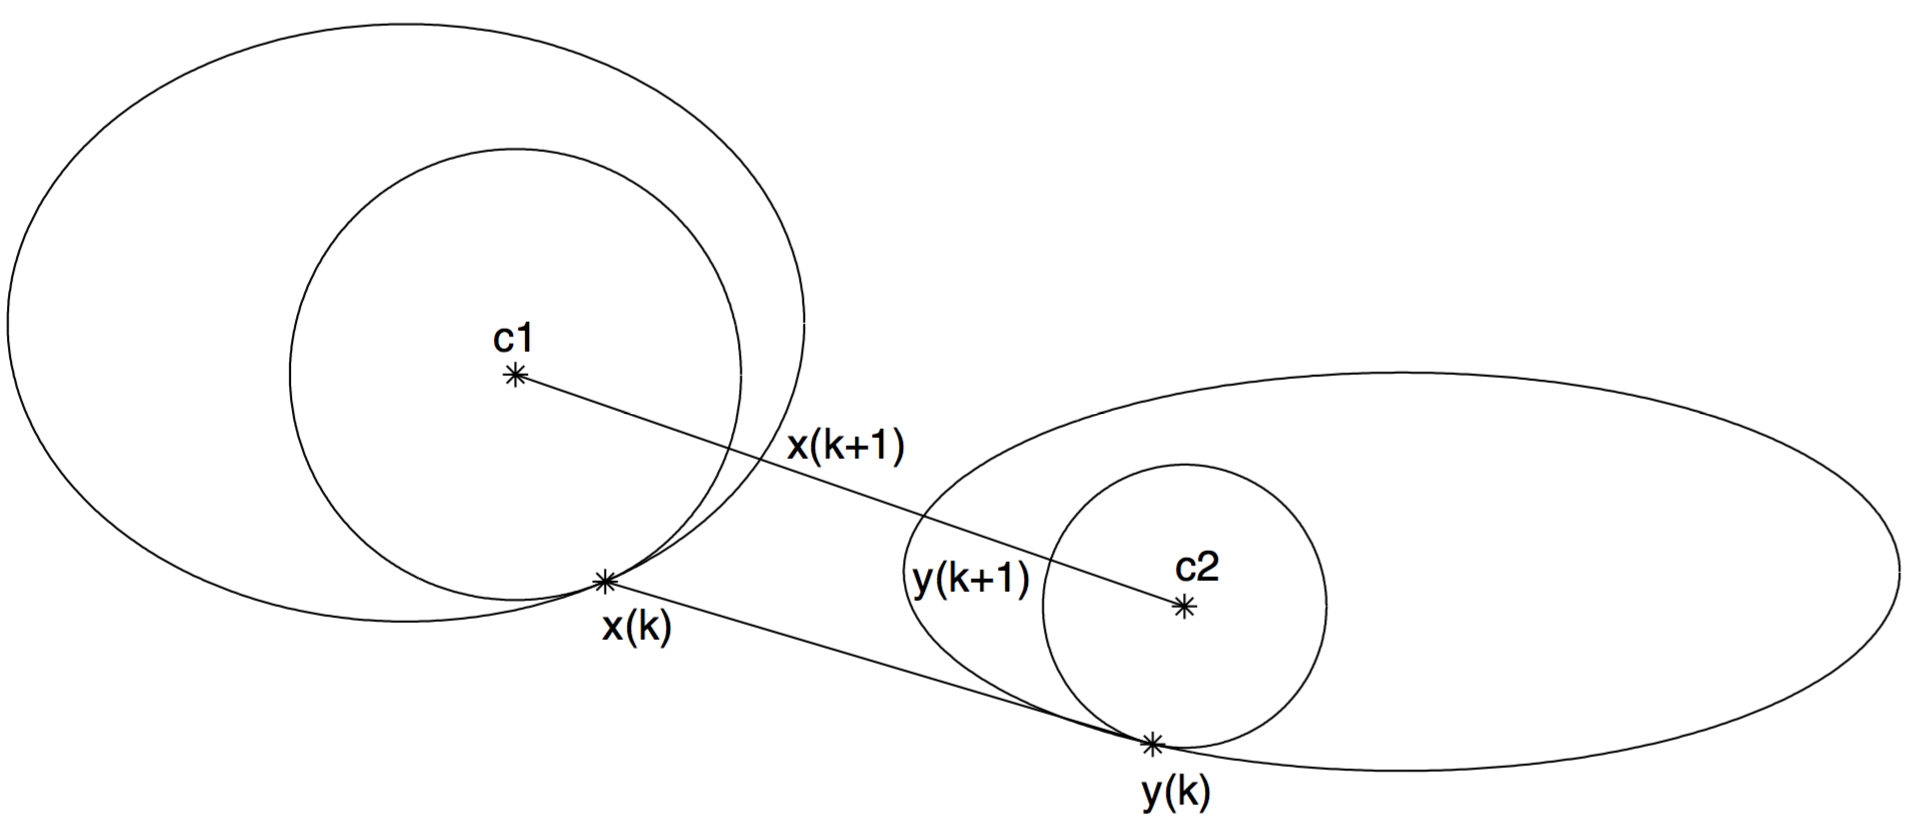
\includegraphics[width=0.5\textwidth]{balls.png}
\caption{\textit{source:} \cite{lin2002distance}}
\label{balls}
\end{figure}

We then check that the line segment $[c_1,c_2]$ is entirely contained in $\mathcal{A}\cup\mathcal{B}$:
\begin{itemize}
\item if it is, then $\mathcal{A}$ and $\mathcal{B}$ are overlapping and therefore $d(\mathcal{A},\mathcal{B}) = 0$ according to its definition in equation \ref{distance_definition},
\item if it is not, we continue and compute the new points $x_{k+1}$ and $y_{k+1}$ which are the intersections of the segment line $[c_1,c_2]$ with $\mathcal{A}$ and $\mathcal{B}$ respectively.
\end{itemize}
The authors of \cite{lin2002distance} have shown that
\begin{equation}
\theta_1 \equiv  (y_{k+1} - x_{k+1};B_{\mathcal{A}}x_{k+1}) = \theta_2 \equiv (x_{k+1} - y_{k+1};B_{\mathcal{B}}y_{k+1}) = 0 \Leftrightarrow d(\mathcal{A},\mathcal{B}) = ||x_{k+1} - y_{k+1}||
\end{equation}
We then have to check for that condition by computing $\theta_1$ and $\theta_2$.

\subsubsection{Construction of the balls}

We need to determine the aforementioned radii and centres of the balls, $r_1,c_1$ and $r_2,c_2$.\\

Since the balls have to be tangent to their belonging matrix, we must have that at the k\textsuperscript{th} iteration $c_1 = x_k - r_1 \vec{n_{\mathcal{A}}}(x_k)$ and $c_2 = y_k - r_2 \vec{n_{\mathcal{B}}}(y_k)$. Our problem is then to find, for a given ellipsoid $\mathcal{E}$ of reduced belonging matrix $\bar{B}_{\mathcal{E}}$, centre $\vec{v}$ and semi-axes $(R_i^{(\mathcal{E})})_{i=1:3}$, a positive real $r$ which satisfies $\forall \vec{r} \in \bar{\mathcal{E}}$, $B(\vec{r} - r\vec{n_{\mathcal{E}}}(\vec{r}),r) \subseteq \mathcal{E}$.\\

We can show that
\begin{equation}
\boxed{\forall \gamma \in \mathbb{R}, 0 < \gamma \leq \frac{1}{\rho(\bar{B}_{\mathcal{E}})}, \forall \vec{r} \in \bar{\mathcal{E}}$, $B(\vec{r} - \gamma \bar{B}_{\mathcal{E}}(\vec{r} - \vec{v}),\gamma ||\bar{B}_{\mathcal{E}}(\vec{r} - \vec{v})||) \subseteq \mathcal{E}}
\end{equation}
with $\rho(\bar{B}_{\mathcal{E}})$ the spectral radius \cite{wiki:spectral} of $\bar{B}_{\mathcal{E}}$. According to equation \ref{reduced_belonging_matrix_}, we have that $\text{sp}(\bar{B}_{\mathcal{E}}) = ((R_i^{(\mathcal{E})})^{-2})_{i=1:3}$ therefore $\boxed{\rho(\bar{B}_{\mathcal{E}}) = \max((R_i^{(\mathcal{E})})^{-2})_{i=1:3}}$.\\

To do so, we have to show that $\forall \vec{r} \in \bar{\mathcal{E}}, \forall \vec{u} \in B(\vec{r} - \gamma \bar{B}_{\mathcal{E}}(\vec{r} - \vec{v}),\gamma ||\bar{B}_{\mathcal{E}}(\vec{r} - \vec{v})||), \vec{u} \in \mathcal{E} \Leftrightarrow (\vec{u} - \vec{v})^T\bar{B}_{\mathcal{E}}(\vec{u} - \vec{v}) \leq 1$ according to equation \ref{reduced_belonging_definition_}.\\

First, we can notice that $\forall \vec{r} \in \bar{\mathcal{E}}, \forall \vec{u} \in B(\vec{r} - \gamma \bar{B}_{\mathcal{E}}(\vec{r} - \vec{v}),\gamma ||\bar{B}_{\mathcal{E}}(\vec{r} - \vec{v})||)$,
\begin{align*}
(\vec{u} - \vec{r})^T\bar{B}_{\mathcal{E}}(\vec{u} - \vec{r}) =& ((\vec{u} - \vec{v}) - (\vec{r} - \vec{v}))^T\bar{B}_{\mathcal{E}}((\vec{u} - \vec{v}) - (\vec{r} - \vec{v}))\\
=& (\vec{u} - \vec{v})^T\bar{B}_{\mathcal{E}}(\vec{u} - \vec{v}) ~\underbrace{- (\vec{u} - \vec{v})^T\bar{B}_{\mathcal{E}}(\vec{r} - \vec{v}) - (\vec{r} - \vec{v})^T\bar{B}_{\mathcal{E}}(\vec{u} - \vec{v})}_{-2(\vec{u} - \vec{v})^T\bar{B}_{\mathcal{E}}(\vec{r} - \vec{v})} + \cancelto{1}{(\vec{r} - \vec{v})^T\bar{B}_{\mathcal{E}}(\vec{r} - \vec{v})}\\
\Leftrightarrow (\vec{u} - \vec{v})^T\bar{B}_{\mathcal{E}}(\vec{u} - \vec{v}) =& (\vec{u} - \vec{r})^T\bar{B}_{\mathcal{E}}(\vec{u} - \vec{r}) + 2(\underbrace{\vec{u} - \vec{v}}_{\mathclap{(\vec{u} - \vec{r}) + (\vec{r} - \vec{v})}})^T\bar{B}_{\mathcal{E}}(\vec{r} - \vec{v}) - 1\\
=& (\vec{u} - \vec{r})^T\bar{B}_{\mathcal{E}}(\vec{u} - \vec{r}) + 2(\vec{u} - \vec{r})^T\bar{B}_{\mathbb{E}}(\vec{r} - \vec{v}) + 2\cancelto{1}{(\vec{r} - \vec{v})^T\bar{B}(\vec{r} - \vec{v})} - 1\\
=& (\vec{u} - \vec{r})^T\bar{B}_{\mathcal{E}}(\vec{u} - \vec{r}) + 2(\vec{u} - \vec{r})^T\bar{B}_{\mathbb{E}}(\vec{r} - \vec{v}) + 1
\end{align*}

From Cauchy-Schwarz inequality we can infer
\begin{align*}
|(\vec{u} - \vec{r})^T\bar{B}_{\mathcal{E}}(\vec{u} - \vec{r})| = |(\vec{u} - \vec{r})\cdot \bar{B}_{\mathcal{E}}(\vec{u} - \vec{r})| \leq ||(\vec{u} - \vec{r})||~||\bar{B}_{\mathcal{E}}(\vec{u} - \vec{r})||
\end{align*}
Let $(\vec{f_i})_{i=1:3}$ be the eigenvectors of $\bar{B}_{\mathcal{E}}$ and $(\lambda_i)_{i=1:3}$ the associated eigenvalues, then
\begin{align*}
\exists (\mu_i)_{i=1:3} \in \mathbb{R}^3, \vec{u} - \vec{r} = \sum_{i=1}^3 \mu_i \vec{f_i}
\end{align*}
and
\begin{align*}
\bar{B}_{\mathcal{E}}(\vec{u} - \vec{r}) = \sum_{i=1}^3 \lambda_i \mu_i \vec{f_i}
\end{align*}
From the definition of the spectral radius \cite{wiki:spectral}, we have that $\forall i \in \llbracket1,3\rrbracket, \lambda_i \leq \rho(\bar{B}_{\mathcal{E}})$ so
\begin{align*}
||\bar{B}_{\mathcal{E}}(\vec{u} - \vec{r})|| &= ||\sum_{i=1}^3 \lambda_i \mu_i \vec{f_i}||\\
&\leq \rho(\bar{B}_{\mathcal{E}})\underbrace{||\sum_{i=1}^3 \mu_i \vec{f_i}||}_{||\vec{u} - \vec{r}||}
\end{align*}
therfore
\begin{align*}
|(\vec{u} - \vec{r})^T\bar{B}_{\mathcal{E}}(\vec{u} - \vec{r})| &\leq ||(\vec{u} - \vec{r})||~||\bar{B}_{\mathcal{E}}(\vec{u} - \vec{r})||\\
&\leq \rho(\bar{B}_{\mathcal{E}}) ||\vec{u} - \vec{r}||^2\\
\Rightarrow (\vec{u} - \vec{r})^T\bar{B}_{\mathcal{E}}(\vec{u} - \vec{r}) &\leq \rho(\bar{B}_{\mathcal{E}}) ||\vec{u} - \vec{r}||^2
\end{align*}
Moreover, since that $\vec{u} \in B(\vec{r} - \gamma \bar{B}_{\mathcal{E}}(\vec{r} - \vec{v}),\gamma ||\bar{B}_{\mathcal{E}}(\vec{r} - \vec{v})||)$, we can write
\begin{align*}
&||\vec{u} - \vec{r} + \gamma \bar{B}_{\mathcal{E}}(\vec{r} - \vec{v})||^2 \leq \gamma^2 ||\bar{B}_{\mathcal{E}}(\vec{r} - \vec{v})||^2\\
\Leftrightarrow &||\vec{u} - \vec{r}||^2 + 2(\vec{u} - \vec{r})^T\gamma \bar{B}_{\mathcal{E}}(\vec{r} - \vec{v}) + \cancel{\gamma^2 ||\bar{B}_{\mathcal{E}}(\vec{r} - \vec{v})||^2} \leq \cancel{\gamma^2 ||\bar{B}_{\mathcal{E}}(\vec{r} - \vec{v})||^2}\\
\Leftrightarrow &(\vec{u} - \vec{r})^T \bar{B}_{\mathcal{E}}(\vec{r} - \vec{v}) \leq -\frac{1}{2\gamma} ||\vec{u} - \vec{r}||^2
\end{align*}
Finally, we then have that
\begin{align*}
(\vec{u} - \vec{v})^T\bar{B}_{\mathcal{E}}(\vec{u} - \vec{v}) &= (\vec{u} - \vec{r})^T\bar{B}_{\mathcal{E}}(\vec{u} - \vec{r}) + 2(\vec{u} - \vec{r})^T\bar{B}_{\mathcal{E}}(\vec{r} - \vec{v}) + 1\\
&\leq \rho(\bar{B}_{\mathcal{E}}) ||\vec{u}-\vec{r}||^2 - \cancel{2}\frac{1}{\cancel{2}\gamma}||\vec{u}-\vec{r}||^2 + 1\\
&\leq ||\vec{u} - \vec{r}||^2\left(\rho(\bar{B}_{\mathcal{E}}) - \frac{1}{\gamma}\right) + 1
\end{align*}
We chose $\gamma$ such that $\gamma \leq \frac{1}{\rho(\bar{B}_{\mathcal{E}})} \Leftrightarrow \rho(\bar{B}_{\mathcal{E}}) \leq \frac{1}{\gamma} \Leftrightarrow \rho(\bar{B}_{\mathcal{E}}) - \frac{1}{\gamma} \leq 0$, therefore $(\vec{u} - \vec{v})^T\bar{B}_{\mathcal{E}}(\vec{u} - \vec{v}) \leq 1 \Leftrightarrow \vec{u} \in \mathcal{E}$.\\

We now have a condition to chose the radius of the balls that have to be constructed in the algorithm. One can notice that this condition is independent of the iteration, therefore we can construct balls that will always be the same size.

\subsubsection{Intersection of the line segment with the ellipsoids}

\paragraph{Authors' method}\mbox{}\\

We need to check if the line segment $[c_1,c_2]$ is entirely contained in $\mathcal{A} \cup \mathcal{B}$ and if so, determine the intersections of this segment with both ellipsoids.\\

To do so, the authors of \cite{lin2002distance} compute $t_1$ and $t_2$ defined as
\begin{equation}
\begin{aligned}
&t_1 = \max\{t \in [0,1], (1-t)c_1 + tc_2 \in \mathcal{A} \Leftrightarrow \mathcal{F}_{\mathcal{A}}((1-t)c_1 + tc_2) \leq 0\}\\
&t_2 = \min\{t \in [0,1], (1-t)c_1 + tc_2 \in \mathcal{B} \Leftrightarrow \mathcal{F}_{\mathcal{B}}((1-t)c_1 + tc_2) \leq 0\}
\end{aligned}
\label{t1_t2}
\end{equation}
\begin{itemize}
\item if $t_2 \leq t_1$, the intersection of $\mathcal{A}$ and $\mathcal{B}$ is non-empty and therefore $d(\mathcal{A},\mathcal{B}) = 0$,
\item if $t_2 > t_1$, we have $\bar{x} = (1 - t_1)c_1 + t_1c_2$ and $\bar{y} = (1 - t_2)c_1 + t_2c_2$ the intersections of the line segments with ellipsoids $\mathcal{A}$ and $\mathcal{B}$ respectively.
\end{itemize}

\paragraph{Polynomial method}\mbox{}\\

The authors' method is essentially numerical, furthermore it makes no use of the information that provides the values of the belonging functions. The following method gives the exact value of the coefficients $t_1$ and $t_2$ introduced in equation \ref{t1_t2}.\\

We want to determine the intersections $r_1$ and $r_2$ of the line segment $[c_1,c_2]$ with ellipsoids $\mathcal{A}$ and $\mathcal{B}$ respectively, whose centres are located in $v_1$ and $v_2$ and whose reduced belonging matrix are $\bar{B}_1$ and $\bar{B}_2$.\\

We will introduce $\alpha_i > 0$ such that
\begin{align*}
r_i &= c_i + \alpha_i(c_j - c_i)\\
\Leftrightarrow r_i - v_i &= c_i - v_i + \alpha_i(c_j - c_i)
\end{align*}
then, according to equation \ref{reduced_belonging_definition_},
\begin{align*}
(r_i - v_i)^T\bar{B}_i(r_i - v_i) &= 1\\
&= (c_i - v_i + \alpha_i(c_j - c_i))^T\bar{B}_i(c_i - v_i + \alpha_i(c_j - c_i))\\
&= \underbrace{(c_i - v_i)^T\bar{B}_i(c_i - v_i)}_{\mathcal{F}_i(c_i) + 1} + 2 \alpha_i (c_i - v_i)^T\bar{B}_i(c_j - c_i) + \alpha_i^2(c_j - c_i)^T\bar{B}_i(c_j - c_i)\\
\Leftrightarrow 0 &= \alpha_i^2(\underbrace{c_j - c_i}_{\vec{a_i}})^T\bar{B}_i(\underbrace{c_j - c_i}_{\vec{a_i}}) + 2\alpha_i (\underbrace{c_i - v_i}_{\vec{b_i}})^T\bar{B}_i(\underbrace{c_j - c_i}_{\vec{a_i}}) + \mathcal{F}_i(c_i)
\end{align*}
therefore, $\alpha_i$ is a root of the polynomial
\begin{align*}
p_i(x) = x^2 \vec{a_i}^T\bar{B}_i\vec{a_i} + 2x \vec{b_i}^T\bar{B}_i\vec{a_i} + \mathcal{F}_i(c_i)
\end{align*}
We can calculate the discriminant $\Delta_i$ of $p_i$
\begin{align*}
\Delta_i = (2\vec{b_i}^T\bar{B}_i\vec{a_i})^2 - 4\vec{a_i}^T\bar{B}_i\vec{a_i}\mathcal{F}_i(c_i)
\end{align*}
where $\bar{B}_i$ is positive definite matrix according to equation \ref{reduced_belonging_matrix_}, therefore $\vec{a_i}\bar{B}_i\vec{a_i} \geq 0$, and $c_i$ is in the corresponding ellispoids, therefore $\mathcal{F}_i(c_i) \leq 0$, which finally leads to
\begin{align*}
\Delta_i \geq (2\vec{b_i}^T\bar{B}_i\vec{a_i})^2 \geq 0
\end{align*}
so $p_i$ has two real roots
\begin{align*}
x_{\pm} = \frac{-2\vec{b_i}^T\bar{B}_i\vec{a_i} \pm \sqrt{\Delta_i}}{2\vec{a_i}^T\bar{B}_i\vec{a_i}}
\end{align*}
of which only $x_+$ is positive, therefore
\begin{equation}
\boxed{\alpha_i = \frac{-2\vec{b_i}^T\bar{B}_i\vec{a_i} + \sqrt{(2\vec{b_i}^T\bar{B}_i\vec{a_i})^2 - 4\vec{a_i}^T\bar{B}_i\vec{a_i}\mathcal{F}_i(c_i)}}{2\vec{a_i}^T\bar{B}_i\vec{a_i}}}
\end{equation}
We have that $\alpha_i$ is maximum when $\mathcal{F}_i(c_i)$ is minimum, which is when
\begin{align*}
\mathcal{F}_i(c_i) = -1 \Rightarrow c_i = v_i \Rightarrow \begin{cases} &\vec{b_i} = \vec{0} \\ &\vec{a_i} = c_j - v_i \end{cases}
\end{align*}
where $c_j$ is not in the ellipsoid of centre $v_i$, therefore $\vec{a_i}\bar{B}_i\vec{a_i} \geq 1$, which leads to
\begin{align*}
\alpha_{i,\text{max}} = \frac{\sqrt{\vec{a_i}^T\bar{B}_i\vec{a_i}}}{\vec{a_i}^T\bar{B}_i\vec{a_i}} \leq 1
\end{align*}
therefore
\begin{equation}
0 \leq \alpha_i \leq 1
\end{equation}

According to equation \ref{t1_t2}, we have that
\begin{align*}
(\cancel{1}-t_1)c_1 + t_1c_2 = r_1 = \cancel{c_1} + \alpha_1(c_2 - c_1) &\Leftrightarrow t_1(c_2 - c_1) = \alpha_1(c_2 - c_1)\\
(1 - t_2)c_1 + t_2c_2 = r_2 = c_2 + \alpha_2(c_1 - c_2) &\Leftrightarrow t_2(c_2 - c_1) = (1-\alpha_2)(c_2 - c_1)
\end{align*}
where $c_2 - c_1 \neq \vec{0}$, therefore
\begin{equation}
\boxed{
\begin{aligned}
t_1 &= \alpha_1 &\in [0,1]\\
t_2 &= 1 - \alpha_2 &\in[0,1]
\end{aligned}
}
\end{equation}

\subsection{Overlapping condition}
\label{distance_intersection}

Since we have the equivalence $\mathcal{A}\cap\mathcal{B} \neq \emptyset \Leftrightarrow d(\mathcal{A},\mathcal{B}) = 0$ according to equation \ref{distance_definition}, we can check if two ellipsoids are overlapping by computing their distance.

% \section{Interactions between two moving ellipsoids}

% In this section, we mean to give an equivalent formulation of the elastic and dissipative forces exerted by two moving spheres on each other\cite{vaagberg2017shear} for ellipsoids.

% \addcontentsline{toc}{section}{References}
\bibliographystyle{unsrtnat}
\bibliography{references/biblio}
{\renewcommand{\bibname}{References}\bibliography{references/biblio}}

\end{document}

% \end{cbunit}